\documentclass[12pt]{article}

\usepackage[margin=1in]{geometry}
\usepackage{amsmath}
\usepackage{graphicx}
\usepackage{mathtools}
\usepackage{color}
\usepackage{relsize}
\usepackage{amssymb}
\usepackage{bm}
\usepackage{listings}
\usepackage{outlines}
\usepackage{enumitem}
\setenumerate[1]{label=\Roman*.}
\setenumerate[2]{label=\Alph*.}
\setenumerate[3]{label=\roman*.}
\setenumerate[4]{label=\alph*.}
\usepackage{threeparttable}
\usepackage{booktabs}
\usepackage{natbib}
\usepackage{setspace}
\usepackage{amsmath}
\usepackage{nccmath}
\usepackage{caption}
\usepackage{subcaption}

\DeclareMathOperator*{\argmax}{arg\,max}
\DeclareMathOperator*{\argmin}{arg\,min}

\usepackage{amsthm}

\newtheorem{assumption}{Assumption}
\newtheorem{theorem}{Theorem}
\let\origtheassumption\theassumption
\doublespacing

\title{Improved Double Machine Learning Estimation for Multivariate Outcomes}

\author{Kyle Colangelo\\University of California Irvine}
\begin{document}


\maketitle
\begin{abstract}
	I propose a new approach to improve the double machine learning (DML) estimator for the case of multi-variate outcomes. The new approach takes advantage of the relationships between outcomes to improve efficiency. This is accomplished in two ways, first through the use of multi-task learning and transfer learning algorithms to learn the nuisance parameters $\eta_0$ more precisely. Second, for a given nuisance estimator we propose an averaging estimator which takes advantage of similarities between causal objects of interest. Various approaches are implemented in Monte Carlo simulations and empirical application which demonstrate the effectiveness of the new method. 
	\\
	\\
	\textbf{Keywords}: 
	%continuous treatment, double debiased machine learning, 
	\\
	\textbf{JEL Classification}: C14, C21, C31, C55
\end{abstract}

\newpage
\section{Introduction}
	 Over the past few years it has been shown increasingly that a wide array of machine learning algorithms have applications not just in predictive modeling, but also in matters of causal inference. Of special note is the double machine learning (DML) estimator developed in \cite{chernozhukov2018double} which provides a general framework for the estimation of a variety of causal parameters in a high-dimensional setting via machine learning. There has been a growing literature surrounding DML, however no attention has been given to the case of multi-variate outcomes. 
	 
	The primary goal of this paper can be stated as to investigate how the DML estimator can be refined to improve efficiency when considering multiple outcomes of interest. Two approaches and their combination are considered: First, by estimating the nuisance parameters using machine learning algorithms which take advantage of the relationships between outcome equations, namely transfer learning and multi-task learning. Second, by implementing a stein-type averaging estimator similar to \cite{hansen2016efficient}, which was extended to Seemingly Unrelated Regression (SUR) in \cite{mehrabani2020improved}.
	
	
	
	 Multitask Learning: In \cite{caruana1997multitask} "Multitask Learning is an approach to inductive transfer that improves generalization by using the domain information contained in the training signals of related tasks as an inductive bias. It does this by learning tasks in parallel while using a shared representation; what is learned for each task can help other tasks be learned better."
	
	Transfer Learning: In the machine learning literature \cite{pratt1993discriminability}. In 2016, Andrew Ng, an industry leading machine learning and AI researcher, stated that transfer learning will be the next driver of industry success. \cite{maurer2016benefit} show the benefit of considering multiple outcomes concurrently with multi-task learning. 
	
	Naturally the potential gains will be widely varied depending on a number of factors. 
	
	In this paper I investigate extensions and usage of the DML estimator for the case of multi-variate outcomes of interest. Specifically, the non-parametric estimation of the average treatment effect (ATE) and the slope coefficient in the partial linear model (PLM) are considered. 
	
	The new approach is analogous to the Seemingly Unrelated Regression (SUR) model in \cite{zellner}.
	
	As a further refinement, an averaging estimator similar to \cite{mehrabani2020improved} is also derived an implemented. 
	
	Recent developments have shown that machine learning methods can be used effectively for a variety of causal inference problems. In particular, \cite{chernozhukov2018double} developed the Double/Debiased machine learning (DML) estimator, which is capable of estimating a variety of causal objects of interest with the proper construction of moment conditions. For example, the DML estimator allows for the estimation of the slope coefficient in the partial linear model, and also the average treatment effect (ATE) for the binary case (the ATE estimation has since been extended to the continuous case in \cite{su2019non} and \cite{colangelo2020double}).
	
	Consider an outcome of interest $Y$, treatment $T$ (allowed to be multi-dimensional), covariate set $X$, and error $\varepsilon$. We may be interested in a nonparametric outcome equation
	\begin{align}
	Y = g(T,X) + \varepsilon\label{eq:1},
	\end{align}
	which also encompasses parametric equations as special cases (such as the partial linear model from \cite{robinson1988root}). 
	
	In many applications we may wish to study the relationship between treatments and multiple different outcomes of interest. If we consider $m$ outcomes of interest, we can extend equation \ref{eq:1} for all $m$ outcomes:
	\begin{align*}
	& Y_1 = g_1(T,X) +\varepsilon_1,\\
	& Y_2 =  g_2(T,X) +\varepsilon_2,\\
	&\vdots\\
	&Y_m =  g_m(T,X) +\varepsilon_m,
	\end{align*}
	where each $g_j$ is allowed to be a different function which may be dependent on a different subset of covariates. The $m$ equations can be stacked together as
	\begin{align}
	\mathbf{Y} = \mathbf{g}(T,X) +\varepsilon\label{eq:2},
	\end{align}  
	Recent developments in the machine learning literature have demonstrated the effectiveness of analyzing multiple outcomes of interest jointly. (see \cite{borchani2015survey}) for a review
	
	This paper not only contributes to the DML literature but also to the non-parametric and semi-parametric estimation literature. While there is a wealth of literature on Seemingly Unrelated Regression (SUR) and multiple equation models, there is very little research on non-parametric estimation of these models. 
	
	When the relationships between outcome equations are non-existent then performing DML equation by equation is optimal. However, in the case where the relationships between outcome equations are strong, efficiency gains can be had by considering them jointly, especially when there is substantial missing data for particular outcomes. 
	
	This paper is organized as follows: I introduce the framework, estimation procedure. Section 3 presents the relevant theoretical results. Section 4 discusses the Monte Carlo simulation results which show the effectiveness of the new estimator. Section 4 provides an empirical demonstration of the new method. Proofs of all results are provided in the appendix. 
\section{Framework}
	\begin{assumption}[Random Sample]\label{as:random} $(Y_i,T_i,X_i)$ are i.i.d.\end{assumption}
	\begin{assumption}[Exogeneity]\label{as:exo} $E(\varepsilon|X) = 0$\end{assumption}
	\begin{assumption}[Error Variance]\label{as:var} 
		$E(\varepsilon_i\varepsilon_j') = \sigma_{ij} I_m$ ($E(\varepsilon\varepsilon') = \Sigma \otimes I_m$) \\
		where $\Sigma =
		\begin{bmatrix}
		\sigma_{11} & \sigma_{12} & \cdots & \sigma_{1m}\\
		\sigma_{21} & \sigma_{22} & \cdots & \sigma_{2m}\\
		&			  &	\vdots & \\
		\sigma_{m1} & \sigma_{m2} & \cdots & \sigma_{mm}
		\end{bmatrix}$
	\end{assumption}
	\begin{assumption}[Unconfoundedness]
		$Y_{1i},Y_{0i}\bot T_i|X_i$
	\end{assumption}
\section{Theory}
\begin{theorem}[Joint Normality-ATE)]\label{norm:ate}
	Under assumptions \ref{as:random}-\ref{as:var}, and the assumptions in \cite{chernozhukov2018double} we have: 
	\begin{align*}
	\sqrt{N}(\hat{\pmb{\beta}} - \pmb{\beta}) \xrightarrow[]{d} N(0,V)
	\end{align*}
	Where
	\begin{align*}
	V = 
	\begin{bmatrix}
	E[\psi_{1i}^2] 	& E[\psi_{1i}\psi_{2i}] & \cdots & E[\psi_{1i}\psi_{mi}] \\
	E[\psi_{2i}\psi_{1i}] & E[\psi_{2i}^2] 	  & \cdots & E[\psi_{2i}\psi_{mi}] \\
	&			  	  &	\vdots & \\
	E[\psi_{mi}\psi_{1i}] & E[\psi_{mi}\psi_{2i}] & \cdots & E[\psi_{mi}^2]
	\end{bmatrix}
	\end{align*}
\end{theorem}

\begin{align*}
	\hat{V} = 
	\begin{bmatrix}
	\frac{1}{N}\sum_{i=1}^N \hat{\psi}_{1i}^2 	& \frac{1}{N}\sum_{i=1}^N \hat{\psi}_{1i}\hat{\psi}_{2i} & \cdots & \frac{1}{N}\sum_{i=1}^N \hat{\psi}_{1i}\hat{\psi}_{mi} \\
	\frac{1}{N}\sum_{i=1}^N \hat{\psi}_{1i}\hat{\psi}_{2i} & \frac{1}{N}\sum_{i=1}^N \hat{\psi}_{2i}^2 	& \cdots  & \frac{1}{N}\sum_{i=1}^N \hat{\psi}_{2i}\hat{\psi}_{mi} \\
	&			  	  &	\vdots & \\
	\frac{1}{N}\sum_{i=1}^N \hat{\psi}_{1i}\hat{\psi}_{mi} & \frac{1}{N}\sum_{i=1}^N \hat{\psi}_{2i}\hat{\psi}_{mi} & \cdots & \frac{1}{N}\sum_{i=1}^N \hat{\psi}_{mi}^2
	\end{bmatrix}
\end{align*}
\section{Simulations}
In this section we evaluate the effectiveness of the previously discussed approaches to double machine learning for multiple outcomes. Two experiments are considered\\
\\
\textbf{Experiment 1:} We consider two outcomes $Y_1$ and $Y_2$ which are fully observed. Nuisance parameters are estimated with multi-task learning.\\
\\
\textbf{Experiment 2:} We consider the same two outcomes, but we allow for $Y_2$ to be missing for 80\% of observations. \\
\\
For both experiments we compare efficiency for the estimation of the average treatment effect for $Y_2$. The following data generating process is used for both experiments:
\begin{align*}
	&\begin{pmatrix}
	\varepsilon_1\\
	\varepsilon_2
	\end{pmatrix} \sim N(0,\Sigma)\\
	&\Sigma = 
	\begin{pmatrix}
		1 & 0.5 \\
		0.5 & 1
	\end{pmatrix}\\
	&X \sim N(\mu,V_x)\\
	&\mu = (1, ..., 1)'\\
	&diag(V_x) = 1\\
	&V_{x,ij} = 0.5 \text{ for } |i-j|=1\\
	&\theta_1 = \mathbf{1}\\
	&\theta_2 = \theta_1 + [\delta,\delta/2,\cdots,\delta/k]\\
	&\beta_1 = 1\\
	&\beta_2 = 1 + \delta\\
	&P(T=1|X) = \Phi\Bigg(\frac{X\theta_1 -\theta_1'\mu}{\theta_1'V_x\theta_1}\Bigg)\\
	&Y_1 = \beta_1T + X\theta_1 + \varepsilon_1\\
	&Y_2 = \beta_2T + X\theta_2 + \varepsilon_2
\end{align*}
We allow $\delta$ to vary between $[0,1]$
\begin{figure}[h!]
	\centering
	\begin{subfigure}{.4\textwidth}
		\centering
		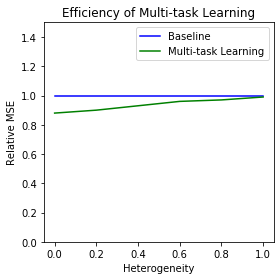
\includegraphics[width=\linewidth]{fig1.png}
		\caption{Relative efficiency of DML with multi-task Learning}
		\label{fig:sub1}
	\end{subfigure}\hfill
	\begin{subfigure}{.4\textwidth}
		\centering
		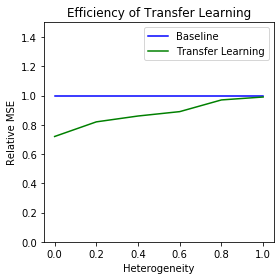
\includegraphics[width=\linewidth]{fig2.png}
		\caption{Relative efficiency of DML with transfer learning}
		\label{fig:sub2}
	\end{subfigure}
	\caption{Results for simulation experiments 1 and 2}
	\label{fig:sim1}
\end{figure}


\section{Empirical Application}
\section{Summary/Conclusion}
\newpage


\appendix


\newpage
\bibliography{references}		% expects file 
\bibliographystyle{aer}	% (uses file "plain.bst")



\end{document}








